\chapter{Fast Data Migration}

%K Scale-out in-memory stores: fast, low-latency, but not immune to load imbalancing and reconfiguration.
The last decade of computer systems research has yielded efficient scale-out
in-memory stores with throughput and access latency thousands of times better
than conventional stores. Today, even modest clusters of these machines can
execute billions of operations per second with access times of 5~\us or
less~\cite{ramcloud,farm-2014}.  These gains come from careful attention to detail
in request processing, so these systems often start with simple
and stripped-down designs to achieve performance goals. For these
systems to be practical in the long-term, they must evolve to include many of the
features that conventional data center and cloud storage systems have
{\em while} preserving their performance benefits.

%K Want operational flexibility of cloud systems, but preserving throughput and latency gains.
To that end, this chapter presents {\em Rocksteady}, a fast migration
and reconfiguration
system for the RAMCloud scale-out in-memory store.  Rocksteady
facilitates cluster
scale-up, scale-down, and load rebalancing with a low-overhead and flexible
approach that allows data to be migrated at arbitrarily fine-grained boundaries and does not
require any normal-case work to partition records.  Measurements show that
Rocksteady can improve the efficiency of clustered accesses and index
operations by more than 4$\times$ (Figure~\ref{fig:cluster-locality}): operations that are common in many
real-world large-scale systems~\cite{fb-memcache,spanner}.  Several works
address the general problem of online (or {\em live}) data migration for
scale-out stores~\cite{slacker,estore,squall,albatross,zephyr,dynamo,spanner},
but hardware trends and the specialized needs of an in-memory key value store
make Rocksteady's approach unique:

\begin{figure}[t]
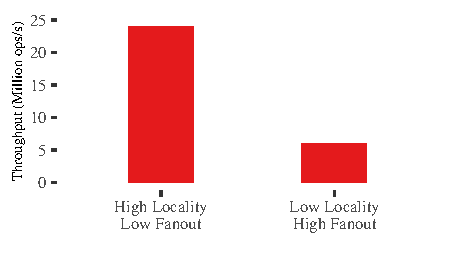
\includegraphics[width=\textwidth]{graphs/migration-motivation.pdf}
\caption{The impact of locality on cluster throughput. When locality is
low due to high fanout, a cluster of RAMCloud servers performs 6 Million
ops/s. On improving locality, by potentially migrating data to reduce
fanout, throughput improves to 24 Million ops/s}
\label{fig:cluster-locality}
\end{figure}


\begin{description}
\item[Low-latency Access Times.]
RAMCloud services requests in 5~\us, and predictable, low-latency operation is
its primary benefit.  Rocksteady's focus is on \nnnth{}-percentile response
times but with 1,000$\times$ lower response times than other tail latency
focused systems~\cite{dynamo}. For clients with high fan-out requests, even
a millisecond of extra tail latency would destroy client-observed
performance. Migration must have minimum impact on access latency
distributions.

\item[Growing DRAM Storage.]
Off-the-shelf data center machines pack 256~to~512~GB per server
with terabytes coming soon. Migration speeds must
grow along with DRAM capacity for load balancing and reconfiguration to be
practical. Today's migration techniques would take hours
just to move a fraction of a single machine's data, making them ineffective for
scale-up and scale-down of clusters.

\item[High Bandwidth Networking.]
Today, fast in-memory stores are equipped with 40~Gbps networks with
200~Gbps~\cite{mellanox-cx6} arriving in 2017. Ideally, with data in memory, these
systems would be able to migrate data at full line rate, but there are many
challenges to doing so.  For example, we find that these network cards (NICs)
struggle with the scattered, fine-grained objects common in in-memory
stores.  Even with the simplest migration
techniques, moving data at line rate would severely degrade
normal-case request processing.

\end{description}

\noindent
In short, the faster and less disruptive we can make migration, the more often we can
afford to use it, making it easier to exploit locality and scaling for efficiency gains.

Besides hardware, three aspects of RAMCloud's design affect Rocksteady's
approach; it is a high-availability system, it is focused on low-latency
operation, and its servers internally (re-)arrange data to optimize memory
utilization and garbage collection. This leads to the following three design
goals for Rocksteady:

\begin{description}
\item[Pauseless.]
RAMCloud must be available at all times~\cite{ramcloud-recovery}, so
Rocksteady can never take tables offline for migration.

\item[Lazy Partitioning.]
For load balancing, servers in most systems
internally pre-partition data
to minimize overhead at migration time~\cite{dynamo,farm-2014}.
Rocksteady rejects this approach for two reasons. First, deferring all
partitioning until migration time lets Rocksteady make partitioning
decisions with full information at hand; it is never constrained by a set
of pre-defined splits. Second, DRAM-based storage is expensive; during
normal operation, RAMCloud's log cleaner~\cite{ramcloud-lsm} constantly
reorganizes data physically in memory to improve utilization and to
minimize cleaning costs. Forcing a partitioning on internal server state
would harm the cleaner's efficiency, which is key to making RAMCloud
cost-effective.

\item[Low Impact With Minimum Headroom.]
Migration increases load on source and target servers. This is particularly
problematic for the source, since data may be migrated away to cope with
increasing load. Efficient use of hardware resources is critical during
migration; preserving headroom for rebalancing directly increases
the cost of the system.

\end{description}

\noindent
Four key ideas allow Rocksteady to meet these goals:
\begin{description}
\item[Adaptive Parallel Replay.]
For servers to keep up with fast networks during migration, Rocksteady fully
pipelines and parallelizes all phases of migration between the source and
target servers. For example, target servers spread incoming data across idle
cores to speed up index reconstruction, but migration operations yield to
client requests for data to minimize disruption.

\item[Exploit Workload Skew to Create Source-side Headroom.] Rocksteady
  prioritizes migration of hot records. For typical skewed workloads, this
  quickly shifts some load with minimal impact, which creates headroom on the
  source to allow faster migration with less disruption.

\item[Lineage-based Fault Tolerance.]
Each RAMCloud server logs updated records in a distributed, striped log which is
also kept (once) in-memory to service requests. A server does not know how its
contents will be partitioned during a migration, so records are intermixed
in memory and on storage. This complicates fault tolerance during
migration: it is expensive to synchronously reorganize on-disk data to move
records from the scattered chunks of one server's log into the scattered chunks
of another's.  Rocksteady takes inspiration from
Resilient Distributed Datasets~\cite{spark}; servers can take dependencies
on portions of each others' recovery logs, allowing them to safely
reorganize storage asynchronously.

\item[Optimization for Modern NICs.]
%Rocksteady is the first data migration mechanism to perform live migrations
%at near-line rate ({\color{red}4~GB/s}) on modern networking hardware, yet it
%preserves SLAs {\color{red} 1,000x} lower than conventional stores.
Fast migration with tight tail latency bounds requires careful attention to
hardware at every point in the design; any ``hiccup'' or extra load results in
latency spikes.
%We profiled modern NICs to
%understand how to best optimize large transfers for the network while
%minimizing impact on host CPU and memory accesses.
%Rocksteady can use kernel-bypass and modern NIC DMA for source-side zero-copy
%of migrated records whenever the hardware supports it;
Rocksteady uses kernel-bypass for low overhead
migration of records;
the result is fast
transfer with reduced CPU load, reduced memory bandwidth load, and more
stable normal-case performance.

\end{description}
